\section{Formation et application d'e-banking}

\subsection{Introduction}

Comme indiqué précédemment, la phase de formation a occupé presque la moitié de mon stage.\\
Cela peut paraître conséquent pour une phase de formation, mais cela fait partie intégrante de l'approche du groupe Excilys concernant les stages de fin d'études.\\

En effet, le stage est orienté dans une optique d'embauche et Excilys tient à ce que les stagiaires et futurs salariés aient une très forte compétence technique sur les technologies Java/JEE, car c'est le segment de marché visé par le groupe :  des clients recherchant des consultants avec  un excellent niveau technique, qui mèneront à bien le projet qu'on leur confie à coup sûr.\\

Seulement, ce niveau de compétence ne peut s'obtenir sans difficultés ou sans y consacrer un temps important. C'est donc pour cette raison que le groupe Excilys a choisi de consacrer autant de temps à cette phase de formation, afin que les stagiaires,futurs consultants, puissent acquérir ces compétences qui leur sont demandées.\\
Le groupe est d'ailleurs très vigilant sur ce point : l'entraide entre stagiaires et consultants est particulièrement encouragée, afin de ne laisser personne en difficulté et les stagiaires sont soumis un mois avant la fin de leur stage à deux entretiens :
\begin{itemize}
	\item un entretien \og d'ingénieur \fg{}, vérifiant que les stagiaires seront en mesure de s'exprimer et de présenter leur travail lorsqu'ils seront en mission chez un client
	\item un entretien technique, vérifiant que les technologies au cœur de la phase de la formation sont parfaitement maîtrisées.  
\end{itemize}

\subsection{Formation Capico}

La première phase de la formation s'est déroulé sur Capico, plateforme d'e-learning développée par Excilys.
J'ai  avons été formés à de nombreuses technologies :
\begin{itemize}
	\item Java/JEE6
	\item UML
	\item Maven
	\item Spring
	\item Hibernate
\end{itemize}

Nous avons également été formé à la méthode \textit{Extreme Programming}, dont certains principes ont été mis en oeuvre pendant le développement de l'application d'e-banking tels que l'intégration continue ou la programmation en binôme.\\

Cette phase de formation a également donné lieu à plusieurs \textit{speechs} donnés par Stéphane LANDELLE, directeur technique d'Excilys, durant lesquelles il a partagé avec nous son expérience du développement Java/JEE afin de nous parler de bonnes pratiques de développement ou de nous présenter plus en détail les technologies au coeur de la formation.

La formation Capico m'a permis de prendre en main ces technologies complexes, avant de les mettre en œuvre dans un projet réel : l'application d'e-banking.

\subsection{Application d'e-banking : MF Banking}

\subsubsection{Fonctionnalités à implémenter}

\begin{tabular}{| c | l | p{8cm} |}
\hline 
Priorité & En tant que XXX\ldots  & je peux\ldots \\ 
\hline 
1 & client authentifié & Consulter sur ma page d'accueil le solde de mes comptes espèce\\ 
\hline 
2 & client authentifié & Consulter le détail d'un compte espèce avec les détails des opérations pour un mois donné. Les opérations carte sont cumulées sur une seule ligne. \\ 
\hline 
3 & client authentifié & Consulter le détail des opération carte pour un mois donné \\ 
\hline 
4 & client authentifié & Réaliser des virements internes \\ 
\hline 
5 & client authentifié & Réaliser des virement externes \\ 
\hline 
6 & internaute & Accéder à ma page de login \\ 
\hline 
7 & internaute & Me logger \\ 
\hline 
8 & client authentifié & exporter au format Excel le relevé des opérations pour un mois donné. Les opérations ne sont pas cumulées.\\ 
\hline 
9 & client authentifié & Consulter l'historique de mes virements \\ 
\hline 
10 & client authentifié & Consulter sur ma page d'accueil l'encours carte sur chacun de mes comptes espèce \\ 
\hline 
11 & client authentifié & Consulter sur ma page d'accueil le solde prévisionnel de chacun de mes comptes espèce \\ 
\hline 
12 & client authentifié & Accéder au détail des opérations carte par un clic sur la ligne de cumul dans le détail des opérations compte \\ 
\hline 
\end{tabular} 

\subsubsection{Méthodologie}

\subsubsection*{Scrum}

Scrum est une méthode de gestion de projet, de la famille des méthodes \textit{agiles}.\\
Les méthodes agiles sont nées du constat que de nombreux projets suivant les méthodes \og conventionnelles \fg{} (telles que le cycle en V) n'étaient pas menés à terme ou généraient d'importants surcouts. Même quand ces projets étaient menés à terme, ils pouvaient être un échec car le besoins du client avaient changé et ces méthodes étaient peu adaptées au changement.\\

Les méthodes agiles telles que Scrum intègrent le client au cœur du processus de  développement en se basant sur des itérations courtes(\textit{sprints}), se concentrant sur un nombre limité de fonctionnalités, au terme desquelles les développeurs doivent pouvoir livrer au client une version incomplète mais parfaitement fonctionnelle.
Celui-ci peut alors apprécier le résultat et demander des changement si besoin est. L'approche choisie par les méthodes agile est d'être réactif aux changements et de s'y adapter plutôt que d'essayer de tout prévoir parfois des années à l'avance.\\

 Le client voit donc son projet évoluer d'itération en itération, au lieu de passer directement d'un cahier des charges à une application terminée.
 
 La méthode Scrum repose principalement sur deux documents : 
 \begin{itemize}
 	\item le \textit{product backlog},liste priorisée des fonctionnalités(ou \textit{items} à réaliser
 	\item le \textit{sprint backlog}, liste des fonctionnalités à réaliser durant le \textit{sprint}\\
 \end{itemize}
 
Il est conseillé d'avoir de petites équipes (une vingtaine de personnes maximum), afin de privilégier la communication entre membres de l'équipe et d'éliminer le besoin de réunions formelles, et auto-organisées, afin de responsabiliser l'équipe (la réussite du projet est la réussite de l'équipe et non d'un chef de projet, mais cela vaut aussi en cas d'échec !)
 Le déroulement d'un \textit{sprint} est le suivant :
 \begin{itemize}
 	\item en accord avec le \textit{Product Owner} (responsable du projet chez le client), on sélectionne les fonctionnalités (qu'on découpe en tâches) qui seront réalisées durant le sprint et on estime le \og coût \fg{} de chaque tâche (temps, difficulté\ldots)
 	\item Quotidiennement se tient le \textit{daily scrum}, qui doit être très bref (environ 1 minute par personne) où on présente ce qu'on a fait la veille, les problèmes rencontrés et ce qu'on pense faire le jour même. Le mieux est de faire du \textit{daily scrum} une routine, en le tenant à chaque fois au même endroit et à la même heure.
 	\item En fin de sprint, on présente au \textit{Product Owner} le résultat du sprint, en ne montrant que ce qui a été terminé. Se tient ensuite la \textit{rétrospective} du sprint , où on fait le point sur l'ensemble du sprint, ce qui est allé, ce qui n'allait pas, les pistes d'amélioration\ldots\\
 \end{itemize}

Dans le cadre de notre application d'e-banking, MF Banking, notre application de la méthode Scrum a été la suivante :
\begin{itemize}
	\item Notre équipe était constituée de 6 personnes
	\item Les \textit{sprints} duraient une semaine, du mercredi au mercredi et le projet s'est étalé sur 5 sprints
	\item Le \textit{daily scrum} se tenait à 10h
	\item La revue technique de notre code par le directeur technique d'Excilys avait lieu le mardi
	\item La revue de l'application par le \textit{Product Owner} avait lieu le mercredi\\
\end{itemize}

La méthode Scrum impose également définir les conditions pour considérer qu'une tâche est terminée (Definition de \og Fini Fini \fg{}). Dans le cadre de l'application d'e-banking, notre définition de \textit{Fini Fini} était la suivante :
\begin{itemize}
	\item Développé
	\item Testé (en local et sur le serveur d'intégration)
	\item Refactoré
	\item Revu par un pair
	\item Documenté (Javadoc)
\end{itemize}

\subsubsection*{Intégration Continue}

L'intégration continue est un processus de développement issu de la méthode \textit{Extreme Programming} (XP). L'un des principes de XP étant de pouvoir à tout moment fournir une version livrable et fonctionnelle au client et l'intégration continue contribue largement au respect de ce principe.

L'intégration continue repose sur quelques grands principes :
\begin{itemize}
	\item Utiliser un logiciel de contrôle de versions
	\item Automatiser le processus de build : des outils comme Maven permettent de compiler, tester et packager le code en une seule commande. On peut également utiliser des serveurs d'intégration continue qui détectent toute modification du dépôt de code et lance automatiquement une build le cas écheant
	\item La build doit être \og auto-testante \fg{} : Dès que le code est compilé, les tests doivent être automatiquement exécutés
	\item La compilation doit rester courte, pour que le résultat soit toujours rapidement visible
	\item Ne pas garder trop de différence entre la version locale et la version sur le dépôt : Ne pas intégrer très régulièrement les modifications peut poser de gros problèmes, l'idéal est de \textit{commit} ses modifications tous les jours
	\item Le résultat de la build doit être visible par tout le monde et les livrables produits facilement accessibles\\
\end{itemize}


\subsubsection*{Build incassable}

Le principe de la build incassable est en quelque sorte une extension de l'intégration continue et repose d'ailleurs sur les outils de l'intégration continue : le contrôle de versions et le serveur d'intégration.\\
Le but de la build incassable est de conserver en permanence le \textit{trunk} (la branche principale) exempt de bugs, en interdisant aux développeurs de mettre directement à jour le \textit{trunk}.

Le principe est le suivant :\\
\begin{figure}
	\centering
		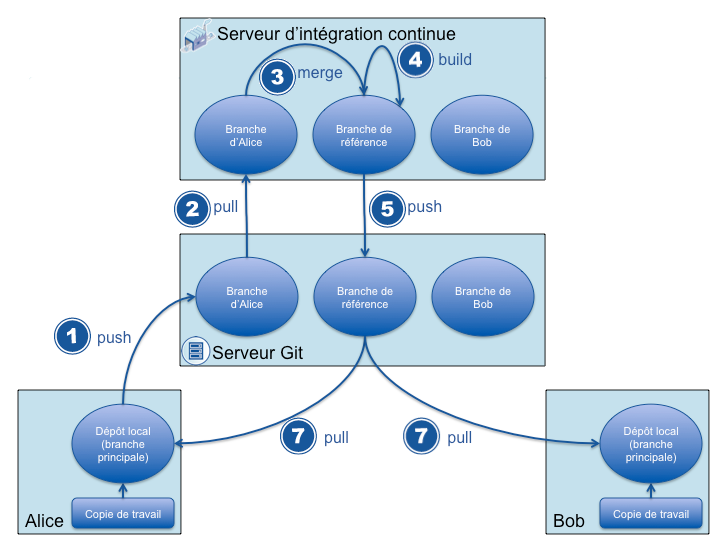
\includegraphics[scale=0.5]{build_incassable.png}
	\caption{Worflow dans un système de build incassable}
\end{figure}

\begin{enumerate}
	\item Chaque développeur dispose d'une \textit{branche}, une version parallèle des sources du dépôt. Quand des modification ont été effectuées et doivent être synchronisées avec le \textit{trunk}, le développeur \textit{push} ses modifications sur sa branche.
	\item Le serveur d'intégration continue détecte les modifications apportées sur la branche du développeur, et récupère ses modifications
	\item	Le serveur d'intégration fusionne alors ces modifications avec sa copie locale du \textit{trunk}
	\item Une build est alors tentée, afin de vérifier que le code compile bien et que l'ensemble des tests passent\ldots
	\item Si la build réussit, le serveur d'intégration propage alors les modification sur le trunk
	\item Les développeurs peuvent alors se synchroniser avec le \textit{trunk}, en étant assuré que l'ensemble est parfaitement fonctionnel
\end{enumerate}
L'inconvénient de la build incassable est qu'elle repose sur le respect de bonnes pratiques de codage de la part des développeurs, notamment l'écriture de tests exhaustifs.\\
En effet, hormis un problème de configuration, un code non testé mais qui compile est une build réussie. Mais un test qui ne passe pas provoque l'échec de la build. Si le code est trop peu ou mal testé, le système de la build incassable perd tout son intêret puisque la build réussira et que du code \og incorrect  \fg{} se retrouvera alors dans la branche principale, pourtant censée ne contenir que du code sûr sur lequel les autres développeurs peuvent s'appuyer sans crainte.  

Dans le cadre de MF Banking, nous avons mis en place un système de build incassable (et d'intégration continue), en se basant sur le système de contrôle de versions Git et le serveur d'intégration Jenkins.\\
A défaut de pouvoir déclencher automatiquement une build lorsqu'une modification était propagée sur le dépôt pour des raisons de configuration réseau, une build était déclenché automatiquement toutes les 15 minutes.

La procédure que nous avons suivi pour mettre en place la build incassable est détaillée sur le blog du cabinet d'expertise informatique Octo\footnote{http://blog.octo.com/gestion-de-version-distribuee-et-build-incassable/}.

\subsubsection{Organisation des sprints}

\begin{itemize}
	\item Sprint 0 et 1:
	\begin{itemize}
		\item Mise en place de l'environnement de développement : Git, Jenkins, SGBD Postgresql et serveur d'applications Tomcat
		\item Mise en place des conventions de codage (nom des classes et méthodes, formatage du code
		 \item Item 1 : \textit{Consulter sur ma page d’accueil le solde de mes comptes espèce}
		 \item Item 6 : \textit{Accéder à ma page de login}
		 \item Item 7 : \textit{Me logger}
		 \item Mise en place d'une page d'administration basique, pour démontrer le bon fonctionnement du système de rôles 
	\end{itemize}
	\item Sprint 2 :
	\begin{itemize}
		\item Item 2 : \textit{Consulter le détail d'un compte espèce avec le détail des opérations pour un mois donné. Les opérations carte sont cumulées sur une seule ligne}
		\item Item 3 : \textit{Consulter le détail des opérations carte pour un mois donné}
		\item Item 12 : \textit{Accéder au détail des opérations carte par un clic sur la ligne de cumul dans le détail des opérations compte}
	\end{itemize}
	\item Sprint 3 : 
	\begin{itemize}
		\item Item 4 : \textit{Réaliser des virements internes}
		\item Item 5 : \textit{Réaliser des virements externes}
		\item Item 8 : \textit{Exporter au format Excel le relevé des opérations pour un mois donné. Les opérations ne sont pas cumulées.}
		\item Item 9 : \textit{Consulter l'historique de mes virements}
		\item Item 10 : \textit{Consulter sur ma page d'accueil l'encours carte sur chacun de mes comptes espèce}
		\item Item 11 : \textit{Consulter sur ma page d'accueil le solde prévisionnel de chacun de mes comptes espèce}
	\end{itemize}
	\item Sprint 4 :
	\begin{itemize}
		\item Ajout de Web Services REST et SOAP
		\item Amélioration de la zone d'administration : ajout de clients, passage de virements\ldots
		\item Mise à jour automatique du solde, du solde prévisionnel et de l'encours carte
		\item Réalisation de deux applications web et d'une application Android pour tester les Web Services
	\end{itemize}
\end{itemize}
\subsubsection{Technologies utilisées}

\subsubsection*{Maven}

Maven est un outil de gestion de projet développé par la fondation Apache.\\
A la différence d'outils tels que Make ou de Ant, son équivalent Java, qui exige de définir précisement les étapes nécessaires à la compilation du code et à la construction du binaire qui en résulte, Maven se base sur un ensemble de conventions (notamment pour l'emplacement du code source, des tests, des ressources de l'application\ldots) qui, si elles sont respectées, permettent de compiler les sources, éxécuter les tests et packager le code compilé avec une configuration minimale. En ce sens, configurer un projet pour qu'il puisse être construit par Maven revient à décrire le projet en lui-m\^eme plus qu'à décrire son processus de compilation.\\

Maven permet également de gérer les dépendances d'un projet (les librairies à utiliser) de façon simple et efficace et son système de plugins permet de l'adapter aux besoins du projet en toute circonstances.\\

Maven se révèle être un outil indispensable, y compris sur des projets de taille réduite. Etant donné le nombre important de librairies utilisées pour l'application MF Banking, le développement de celle-ci se serait averé beaucoup plus complexe sans l'apport de Maven et son système de gestion de dépendances. 

\subsubsection*{Spring}

Spring est un framework destinée aux application d'entreprise, développé par SpringSource.Spring est né en 2003, suite à de multiples déboires avec la solution pour les applications d'entreprise de l'époque, JEE et le EJB.\\

Le coeur du framework Spring est son conteneur IoC (\textit{Inversion of Control}).
D'une certaine façon, l'IoC  (ou, selon l'article de Martin Fowler sur IoC\footnote{http://martinfowler.com/articles/injection.html}, l'injection de dépendances)  est une alternative à l'opérateur \textit{new} : on définit \textbf{par configuration} quelles classes classes devront être instanciées,configurées et gérées par le conteneur (on appelle alors ces instances des \textit{beans} et ces \textit{beans} peuvent être ensuite automatiquement \og injectées \fg{}  dans les classes de l'application à développer et être utilisées telles quelles,sans qu'il y ait besoin de créer soi-même une nouvelle instance.\\
Dans le cas où la classe que l'on souhaite injecter implémente une interface, il est tout à fait possible et même conseillé de ne faire référence qu'à l'interface, le conteneur Spring se chargera alors d'injecter l'implémentation automatiquement.
Cela permet donc d'avoir un couplage réduit au strict minimum, puisque les classes n'ont même pas connaissance de l'implémentation sous-jacente,uniquement connue du conteneur IoC de Spring.\\

L'interêt du framework Spring ne se limite pas à son conteneur IoC et il propose également de nombreuses intégrations avec d'autres technologies, telles que Hibernate/JPA. 

\subsubsection*{Hibernate et JPA}

Hibernate est un ORM (Object-Relationnal Mapper). L'interêt d'un ORM est de s'abstraire du SQL en laissant celui-ci se charger des requêtes SQL à proprement parler.\\
Ceci est possible en configurant la manière dont un objet Java est liée à la base de données (quelle classe correspond à quelle table ? quel variable d'instance correspond à quel attribut ?) et la manipulation de l'objet Java geré par l'ORM aboutira alors à l'éxécution automatiques des requêtes SQL appropriées.\\
JPA (ou Java Persistence API), API issue des spécifications JSR-224 et JSR-317, est justement une manière de configurer la façon dont une classe Java est liée à la base de données, par le biais d'annotations.

\subsubsection*{CXF}

CXF est un framework développé par la fondation Apache, simplifiant l'écriture de Web Services.\\

On peut voir les Web Services comme une moyen de communication entre applications.
Un exemple typique d'utilisation des Web Services est le comparateur de prix. Un comparateur de prix ne va pas stocker directement toutes les informations des différents sites qu'il cible, pour des raisons évidentes : sécurité des informations, synchronisation des bases de données,etc\ldots\\La solution est de faire appel à des Web Services,exposés par les sites marchands, que le comparateur de prix requêtera afin d'obtenir les informations souhaitées. La logique métier de gestion des stocks, des tarifs\ldots restent donc du côté de l'application requêtée.\\

Il nous a été demandé d'implémenter des Web Services SOAP et REST pour MF Banking, et nous avons  utilisé le framework CXF pour les réaliser.

\subsubsection{Architecture}

L'architecture de MF Banking repose sur le modèle de l'architecture $N$-tiers.
Le principe de cette architecture consiste à découper l'application en plusieurs couches (le plus souvent trois couches), chacune ayant un but très précis. Ce découpage présente deux avantages majeurs :
\begin{itemize}
	\item chaque couche ayant un but bien précis, celle-ci est plus facile à maintenir et est aisément découplable du reste de l'application. 
	\item Les couches pouvant facilement être découplées, les couches sont interchangeables
\end{itemize}
Il en résulte une application hautement modulaire, où chaque couche peut (théoriquement) être remplacée ou mise à jour en ayant un impact réduit sur le reste de l'application.\\

Dans le cas d'une architecture 3-tiers, que nous avons utilisé pour MF Banking, les  couches sont les suivantes :

\begin{figure} [h!]
	\centering
		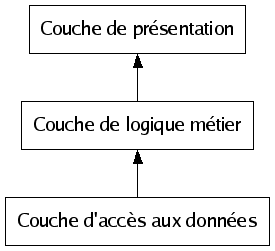
\includegraphics[scale=0.5]{ntiers.png}
	\caption{Architecture 3-tiers}
\end{figure}

Le rôle de la couche d'accès aux données est, comme son nom l'indique, d'accès aux données de l'application. Typiquement, cette couche se charge d'accéder à une base de données et d'y récupérer les informations ou d'en stocker des nouvelles.\\
 Dans notre cas, la couche d'accès aux données accédait à une base de données PostgresSQL, via JPA et Hibernate.\\

La couche de logique métier est le pivot de l'application : c'est dans cette couche qu'est gerée toute la logique propre à l'application que l'on souhaite développer, et sert donc de pont entre les données et la façon dont elles sont présentées à l'utilisateur.\\

Enfin, la couche de présentation est celle qui est en charge d'afficher les données de l'application.\\
 Dans notre cas, la couche de présentation consistait en une série  de pages JSP, gérées par Spring MVC.
 
 Les Web Services SOAP et REST que nous avons mis en place était des couches de présentation alternatives, réutilisant la couche de logique métier.\\
 
 Les frameworks permettant l'injection de dépendances tels que Spring simplifient grandement la mise en place d'architecture n-tiers.\\
 En déléguant le \og câblage \fg{} automatique des implémentations au conteneur Spring et en utilisant systématiquement des interfaces (afin de ne pas dépendre directement d'une implémentation), remplacer une implémentation par une autre revient finalement à fournir la bonne archive JAR contenant les implémentations désirées.  

\subsubsection{Schéma de la base de données}
\begin{figure}[h!]
	\centering
		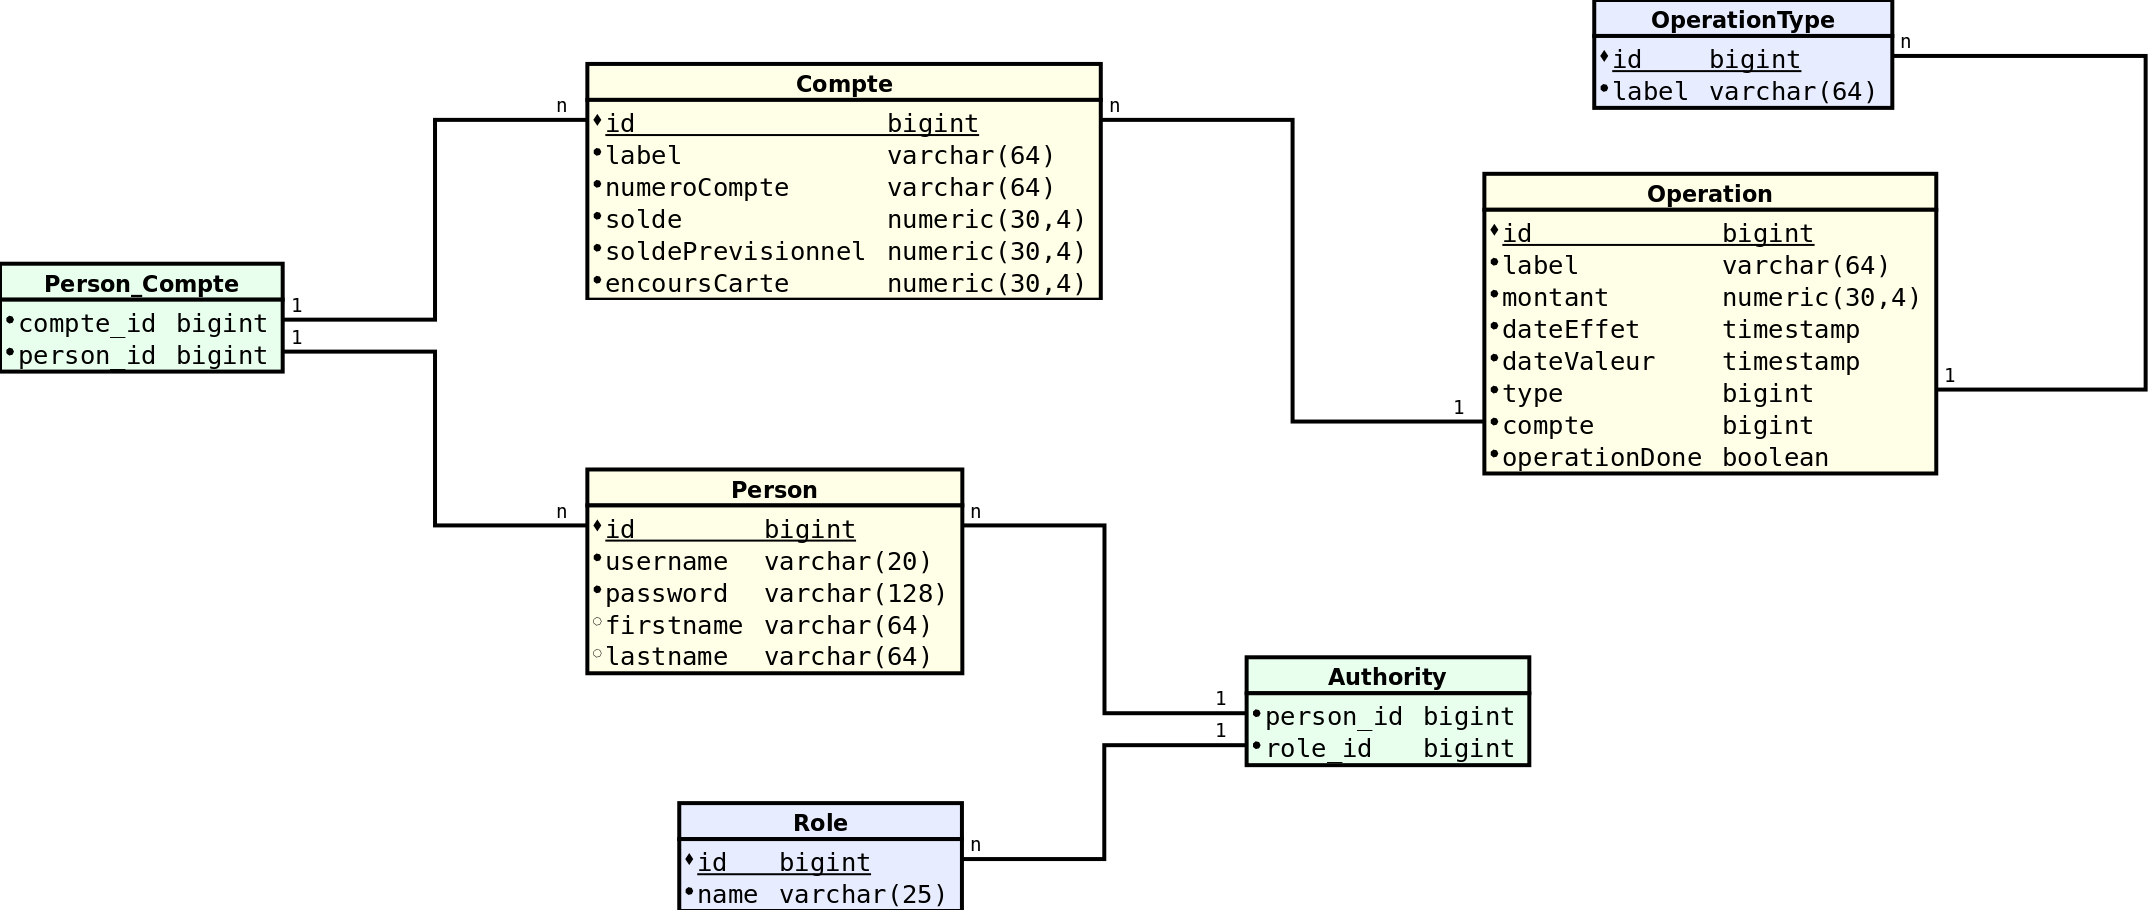
\includegraphics[scale=0.25]{diagramme_modele.png} 
	\caption{Modèle E/A de la base de données}
\end{figure}

Rôles de chaque table :
\begin{itemize}
	\item Person : liste des clients de MF Banking
	\item Role : liste des rôles que peuvent avoir les utilisateurs (client ou administrateur)
	\item Authority : table de jointure entre Person et Role. Il était nécessaire d'avoir une table de jointure car un utilisateur peut être à la fois utilisateur et administrateur,  
	\item Compte : liste des comptes des utilisateurs
	\item Person\_Compte : table de jointure entre Person et Compte. Ici aussi, il était nécessaire d'utiliser une table de jointure car un utilisateur peut avoir plusieurs comptes et les comptes peuvent \^etre des comptes joints
	\item Operation : liste des opérations bancaires effectuées sur les comptes
	\item OperationType : liste des types d'opérations bancaires (chèque, carte bleue, virement et espèce)
\end{itemize}
 \subsubsection{Structure}
Par le biais de Maven, nous avons découpé notre application en plusieurs modules :
\begin{itemize}
	\item Entities
	\item DAO
	\item Services et Services API
	\item Batch
	\item Web
	\item Webservices
	\item Application Android
\end{itemize}

\subsubsection*{module Entities}

Ce module regroupe les différentes entités de notre application, miroir objet de notre base de données ainsi que les scripts Liquibase de mise à jour du schéma de base de données.\\
 La librairie Liquibase nous a permis de construire notre schéma de base de données de manière incrémentale  au fil des ajouts de nouvelles entités ou de nouvelles colonnes. Les mises à jour du schéma étaient  appliqués automatiquement à chaque déploiement de l'application, assurant l'ensemble de l'équipe d'avoir automatiquement un schéma à jour.  Cette approche est également plus compatibles avec les méthodes agiles, en créeant uniquement les tables et colonnes nécessaires pour la fonctionnalité en cours d'écriture, avec la possibilité d'effectuer des modifications quand le besoin s'en fera sentir.\\
 Les tables de jointure n'étant pas représentées par des entités, nous avons donc cinq entités :
 \begin{itemize}
 	\item Person, un utilisateur de MF Banking (qu'il soit simple utilisateur et/ou administrateur)
 	\item Role, les rôles que peut avoir un utilisateur de l'application (utilisateur et administrateur)
 	\item Compte, un compte bancaire d'un utilisateur (avec possibilités d'avoir plusieurs comptes par utilisateur et des comptes joints)
 	\item Operation, une opération (crédit ou débit) sur un compte bancaire
 	\item OperationType, le type d'une opération (virement, chèque, espèce ou carte bleue)
\end{itemize}  

\subsubsection*{module DAO}

Le module DAO correspond à la couche d'accès aux données.\\
DAO est l'acronyme de \textit{Data Access Object} : un DAO est une classe Java dont le but est d'accéder et de modifier les données stockées par l'application. Ce terme est parfaitement générique : que les données soient stockées dans un fichier ou dans une base de données, la classe se chargeant de récupérer ces données reste un DAO.\\ 
Sont centralisés dans ce module l'ensemble de  la configuration Spring ayant trait à l'accès aux bases de données (connexion, infrastructure Hibernate/JPA, gestion des transactions\ldots) ainsi que le code en charge de la récupération des données depuis la base de données, en se basant sur les entités définies dans le module Entities.\\

En production, l'application utilisait une base de données PostgresSQL mais une base de données H2 a été également utilisée pour effectuer des tests unitaires.Cette base, comme les bases Derby et HSQLDB, présente l'avantage de pouvoir fonctionner uniquement en mémoire, ce qui est très adapté dans le cadre de tests unitaires : la base de données est crée, initialisée grâce à Liquibase et des données sont ajoutées le temps d'effectuer les tests unitaires et la base est détruite une fois le test terminé. On a donc des tests unitaires faciles à reproduire, puisqu'ils sont à chaque fois exécutés sur une base de données vierge.\\

Afin de réaliser les tests unitaires, nous nous sommes aidées d'une librairie développée par Stéphane appelée Spring DB-Unit simplifiant grandement l'insertion de données de tests dans la base en mémoire. 

Idéalement, ce module aurait dû être découpé en deux modules, DAO et DAO API, afin de découpler complètement les interfaces et des DAO et leurs implémentations. En l'état, il est théoriquement possible de faire directement référence aux implémentations, bien que cela n'ait pas été fait.\\
 
\subsubsection*{Services et Services API}

Le module Services est le cœur de l'application, où se situe l'ensemble de la logique métier (comment effectuer les virements, quelles vérifications effectuer, comment gérer l'authentification des utilisateurs\ldots).\\
Comme expliqué précédemment, cette couche est le pivot de l'application et c'est donc typiquement la seule couche qui n'est pas remplacée, surtout si le modèle de l'architecture $N$-tiers est correctement implémentée, ce qui est le cas pour MF Banking : le module Service ne dépend aucunement de la façon dont l'accès aux données est implémenté, ni de la façon dont les informations sont présentées à l'utilisateur.\\

Afin de respecter au maximum les bonnes pratiques de codage lié à l'architecture $N$-tiers, nous avons dû tester les services en isolation, sans qu'ils dépendent de s implémentations de la couche DAO. Pour ce faire, nous avons utilisé Mockito, une librairie permettant de créer de \og faux \fg{} objets, dont nous déterminions le comportement, par exemple : \textit{si la méthode X d'un DAO est appelée, alors le résultat Y doit être retourné}.\\
Les tests unitaires des services ne testaient donc QUE les services et nous étions donc assurés qu'en cas de problème, le problème ne pouvait venir en aucun cas de la couche inférieure. 

\subsubsection*{Batch}

Comme pour une véritable banque, les opérations de MF Banking dispose d'une date d'effet (date à laquelle l'opération a été enregistrée) et d'une date de valeur (date à laquelle l'opération est prise en compte et le solde modifié en conséquence).\\

Cette modélisation impose cependant de mettre à jour automatiquement le solde du compte lorsque la date de valeur d'une ou plusieurs opérations correspond au jour courant.\\
Nous avons mis en place cette mise à jour automatique par le biais de Spring Batch : une tâche de mise à jour du solde est exécutée à intervalles réguliers (dans une véritable application d'e-banking, l'exécution devrait avoir lieu toutes les 24 heures, nous avons utilisé des intervalles beaucoup plus courts afin de pouvoir tester plus rapidement la modification).\\
Un flag indique si une opération a été prise en compte ou non et, le cas échéant, le solde est mis à jour et l'opération est marquée comme traitée.

\subsubsection*{Web}

Le module Web correspond à la couche de présentation de l'architecture $N$-tiers.\\
Nous avons utilisé le framework Spring MVC pour bâtir notre couche web, car il offrait de nombreux avantages : Spring MVC est parfaitement intégré à Spring et son modèle de programmation est simple et permet de développer rapidement des interactions complexes avec l'utilisateur. Comme son nom le laisse suggérer, Spring MVC tend à se rapprocher d'une architecture Modèle-Vue-Contrôleur.\\

Le module Web est très nettement le module qui a le plus bénéficié de librairies tierces-parties, toujours dans le but de simplifier autant que possible le développement en déléguant les tâches complexes ou répétitives à une librairie dont c'est la spécialité.\\
Nous avons utilisé entre autres : 
\begin{itemize}
	\item Bootstrap, développé par Twitter, offre un ensemble cohérent de feuilles de style CSS et de code JS permettant de développer simplement une interface web agréable à utiliser. Etant donné que le but de cette formation n'était pas de tester nos compétences HTML/CSS/JS, Bootstrap nous a permis d'avoir une application web élégante sans consacrer trop de temps à l'écriture de feuilles de style CSS.
	\item Tiles, librairie de \textit{templating} développée par la fondation Apache. Notre interface web incluait plusieurs éléments se retrouvant sur l'ensemble des pages : les feuilles de style et les scripts JS de Boostrap, une barre de navigation\ldots Afin d'éviter de réécrire à chaque fois ces mêmes lignes de code, avec le risque de les oublier à l'occasion, Tiles nous a permis de définir un \og modèle \fg{} de page incluant systématiquement ces éléments et nous nous chargions alors d'écrire uniquement les éléments de la page qui différaient.
	\item Hibernate Validator est l'implémentation de référence de la Java Validation API, spécifiée par la JSR-303.Les fonctionnalités offertes par la JSR-303 nous ont permis de simplifier grandement la validation des formulaires de MF Banking. Là où une validation \og classique \fg{} des données consisterait à vérifier manuellement tous les champs du formulaire à valider, la JSR-303 permet par le biais d'annotations de définir les contraintes que doivent respecter un champ d'un formulaire et le support de la JSR-303 par Spring permet de déclencher automatiquement cette validation. Et toujours grâce aux fonctionnalités offertes par Spring, il a été également très simple d'afficher des messages d'erreur internationalisés à chaque fois qu'une erreur de validation du formulaire était survenue.
	\item POI, API gérant l'écriture de documents Word,Excel et Powerpoint, développé par la fondation Apache. Une des fonctionnalités à réaliser était l'export du rélevé des opérations au format Excel. Grâce aux fonctionnalités offertes par POI, la manipulation de documents Excel s'est avérée très aisée et nous a évité d'avoir à manipuler directement le format Excel, ce qui aurait pu s'avérer très complexe.\\
\end{itemize}

Au même titre que les autres couches de notre application, la couche Web n'a pas échappé à des tests automatisés.La nature même des pages web rendant compliqué l'écriture de tests unitaires, nous n'avons pas effectué de tests unitaires vérifiant le comportement de chaque pages de façon isolée.\\
L'approche que nous avons adopté est celle des tests d'intégration : nous avons vérifié le comportement global de l'application en nous assurant qu'un utilisateur pourrait naviguer entre les pages et effectuer toutes les actions qu'il souhaite comme prévu.\\

Pour ce faire, nous avons utilisé l'outil Selenium. Pour citer les auteurs de Selenium, cet outil \og automatise les navigateurs \fg{}. On crée un scénario de test en naviguant sur les différentes pages du site et cette succession de pages est ensuite enregistrée par Selenium, qui convertit ce scénario en code Java.\\
Le principe de Selenium est ensuite assez simple : Selenium démarre un navigateur Web et exécute le scénario de test en simulant les clics et les saisies clavier. Si Selenium réussit à reproduire le scénario de test, le test est réussi. Cela prouve donc qu'aucune fonctionnalité testée n'a été impactée par une modification du code.\\

Afin d'effectuer les tests Selenium dans des conditions optimales, les tests étaient effectuées sur une base de données PostgresSQL à part, remplie avant chaque le lancement des tests et vidée lorsqu'ils terminent. Les résultats étaient donc parfaitement reproductibles, sans risque qu'une mise à jour des données effectuée par les tests  risque de faire échouer un test après de multiples exécutions.
On peut notamment citer le cas des virements, diminuant le solde des comptes à chaque fois, jusqu'au point où le solde pourrait ne plus être suffisant et le virement par conséquent refusé.\\

Afin de ne pas permettre à un utilisateur anonyme d'accéder aux comptes de n'importe quel client de MF Banking, notre application a été évidemment sécurisée.Une fois de plus, nous avons utilisé une librairie développée par Spring : Spring Security.\\
Spring Security permet de s'abstraire d'une large part de la complexité de la sécurisation d'une application, en ne demandant au développeur qu'à préciser ce qui doit \^etre sécurisé,comment cela doit être protégé et qui peut y accéder.
\subsubsection*{WebServices} 

Comme indiqué précedemment, on peut voir les Web Services comme une couche de présentation alternative.\\
Bien qu'ils ne constituent pas un moyen de présenter les données visuellement à l'utilisateur, ils sont néanmoins pour l'application un moyen de communiquer avec l'extérieur, au même titre que des pages web. Au même titre que le module Web, le module Web Services vient réutiliser le modules Services.\\

Nous avons mis en place deux types de Web Services pour MF Banking : des Web Services SOAP et des Web Services REST.\\

Les Web Services SOAP se basent sur l'échange de fichiers XML au format SOAP contenant les informations que les applications doivent se transmettre,en l'occurence les arguments à passer aux méthodes des Web Services et les valeurs qui sont retournées par ces m\^emes méthodes.\\
Les différents services exposés, les types de données acceptés en entrée et retournés sont exposés via un fichier descripteur, au format WSDL (Web Service Definition Language).\\
L'avantage et à la fois l'inconvénient du SOAP est qu'il est basé sur le XML : le WSDL est avant tout un schéma XML et les données fournies au Web Service peuvent être validées grâce au WSDL, évitant ainsi d'envoyer des données incohérentes. Par contre, XML est un format de fichier très verbeux, où la quantité de données \og utiles \fg{} est finalement assez faible à cause des balises XML. \\
L'API Java centré autour de la création de Web Services SOAP se nomme JAX-WS (Java API for XML Web Services) et est standardisé via la spécification JSR-224.
Apache CXF,le framework que nous avons utilisé pour gérer les Web Services, propose deux approches pour générer de nouveaux Web Services ou le code y accédant : 
\begin{itemize}
	\item \textit{code first} : on écrit d'abord le code du Web  Service, et les annotations de JAX-WS fournissent les métadonnées nécessaires à la génération du fichier WSDL correspondant à ce Web Service
	\item \textit{contract first} : on écrit d'abord le WSDL et des outils de génération de code se chargent d'écrire le code du Web Service correspondant. On peut également se servir d'un WSDL existant pour générer le code accédant au Web Service correspondant, épargnant ainsi la manipulation d'un fichier XML au format complexe.\\
\end{itemize}
Nous avons utilisé ces deux approches pour MF Banking :
\begin{itemize}
	\item les Web Services en eux-mêmes étaient \textit{code first}, car nous disposions déjà du code des services (ce qui réduisaient considérablement la quantité de code à écrire) et que l'écriture d'un fichier WSDL s'avérait être une tâche trop complexe à réaliser dans le temps qui nous était imparti.
	\item les WSDL générés ont été réutilisés pour générer le code des clients des Web Services\\
\end{itemize}

Les Web Services REST suivent une approche très différente de celle des Web Services SOAP. L'idée de départ des Web Services REST (REpresentational State Transfer) est de se baser sur les différents \og verbes \fg{} du protocole HTTP pour définir le type d'action réalisée par une méthode d'un Web Service : une requête GET récupère des données, une requête POST ajoute ou met à jour un élement, une requête DELETE supprime un élément\ldots.\\
Contrairement à SOAP, REST ne met pas de contrainte sur le format des données échangées (qui peuvent donc être au format XML si on le souhaite), bien que le format le plus souvent utilisé soit le JSON (Javascript Simple Object Notation), car c'est un format simple et très compact (et qui peut être lu sans utiliser de librairie supplémentaire par du code Javascript).\\
L'exploitation des spécificités du protocole HTTP font que l'accès à un Web Service REST se limite à envoyer une requête HTTP à une URL précise et l'ensemble des services exposés se limite alors à une simple collection d'URLs.\\

Nous avons également utilisé CXF pour créer les Web Services REST de notre application en \textit{code first}. L'approche \textit{contract first} n'a pas été exploitée pour deux raisons :
\begin{itemize}
	\item Bien qu'il existe un schéma XML pour les Web Services REST au format  WADL (Web Application Description Language), il n'est que rarement utilisé et s'avère de toute façon sans intêret lorsque JSON est utilisé comme format d'échange
	\item Etant donné qu'interroger un Web Service REST se limite à effectuer une requête HTTP sur une URL, une librairie simplifiant la construction et l'émission de requêtes HTTP suffit amplement pour interroger un Web Service REST efficacement.
\end{itemize} 

\subsubsection*{Application Android}

L'application Android n'était pas une demande explicite du Product Owner, mais celle nous a permis de mettre en oeuvre les Web Services REST que nous avons implémenté.

\begin{figure}[h!]
	\centering
		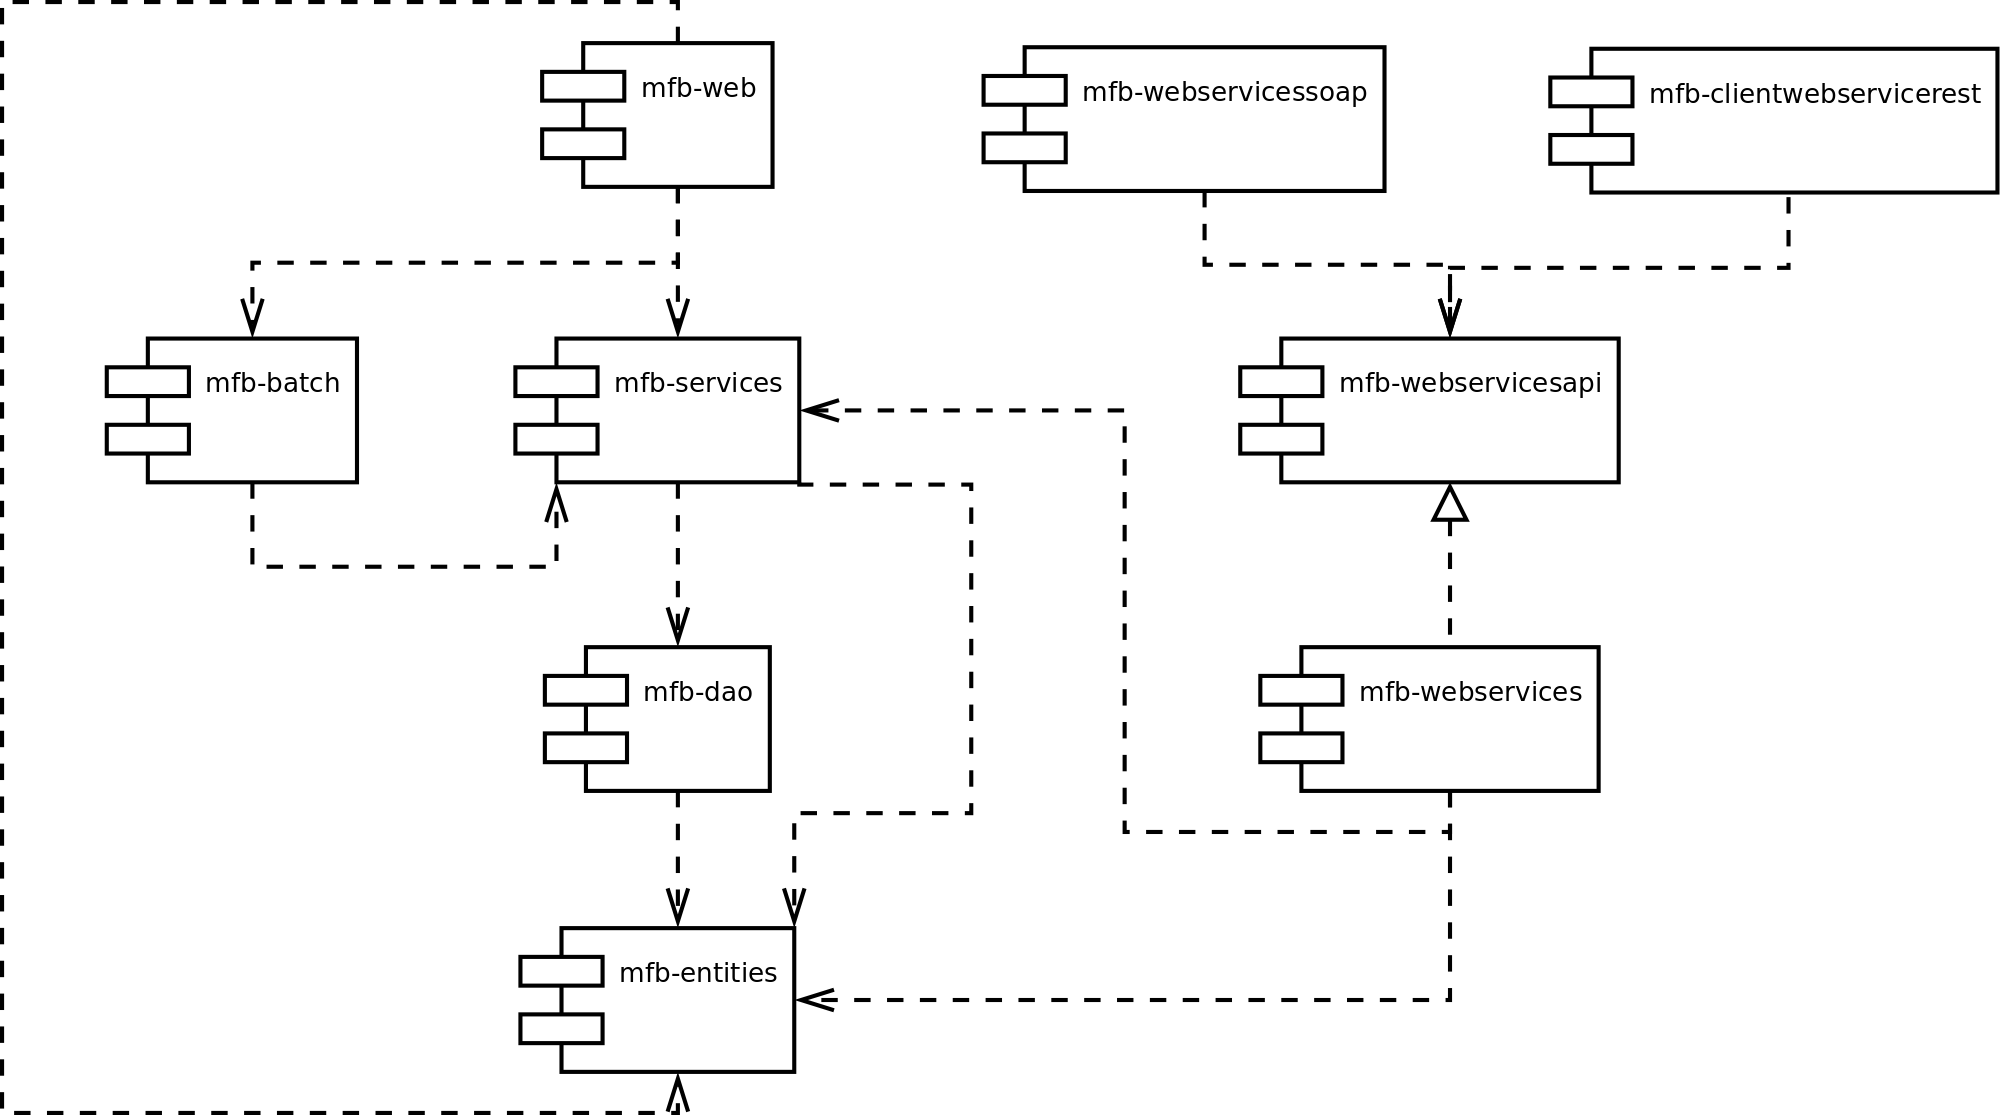
\includegraphics[scale=0.3]{diagramme_modules.png}
	\caption{Interaction entre les différents modules de MF Banking}
\end{figure}

\subsubsection{Apport personnel}

Comme tous les autres membres de mon équipe, j'ai participé au développement de chacune des fonctionnalités de MF Banking.\\
Ma contribution a pris différentes formes :
\begin{itemize}
	\item Séléction des \textit{items} à implémenter au sprint suivant
	\item Modélisation de la base de données quand cela était nécessaire
	\item Recherche de librairies pouvant nous aider dans le développement d'une fonctionnalité et quand la recherche s'est avérée fructueuse, lecture de documentation sur la librarie choisie afin de comprendre comment s'en servir
	\item Développement des fonctionnalités en binôme, que ça soit en tant que codeur ou en tant qu'observateur.
	\item Validation d'une tâche avant que celle-ci soit considerée comme terminée.\\
\end{itemize}

J'ai pris part au développement de chacun des modules et ai donc eu l'occasion de travailler sur l'ensemble des technologies mises en oeuvre dans MF Banking.\\

Si je devais mettre en avant un rôle particulier dans que j'ai joué durant le développement de MF Banking, cela serait la recherche de librairies et leur intégration dans notre projet.\\
Stéphane, durant un de ses \textit{speechs}, a insisté sur l'intérêt d'utiliser des librairies afin d'éviter de réimplémenter des fonctionnalités déjà existantes et bien mieux réalisées que nous aurions pu le faire, ceci afin de se concentrer uniquement sur le code spécifique à notre application.\\
J'ai donc mis ce principe en oeuvre au maximum et, avant de commencer à développer une nouvelle fonctionnalité, mon réflexe fut de chercher systèmatiquement si une librairie  ou plusieurs pourraient nous être utiles, les étudier afin de séléctionner la plus adaptée puis de comprendre son fonctionnement pour la mettre en oeuvre dans MF Banking.\\
J'ai entre autres incité mes collègues à ce que Liquibase, Spring-DBUnit ou Hibernate Validator soient utilisées. 
\subsubsection{MF Banking en chiffres}

En résumé, MF Banking, c'est : 
\begin{itemize}
	\item 6 développeurs
	\item 5 semaines de développement
	\item 444 commits
	\item 8000 lignes de code
\end{itemize}

\subsubsection{Tests de charge sur MF Banking avec Gatling}

Durant mon travail sur Gatling, et afin de le prendre en main, j'ai été amené à écrire un test de charge de MF Banking.\\
Ce test de charge, impliquant l'utilisation simultanée de l'application par 1000 utilisateurs, a montré que notre application résistait bien au test et que notre implémentation était donc suffisamment performante.\\
Ce scénario de test a effectué 110000 requêtes sur MF Banking, donc aucune n'a échoué. Le temps moyen de réponse est de 191 ms, avec un temps de réponse maximal de 9,6 secondes.\\
Les résultats détaillés du tests sont présents en annexe.

\subsubsection{Accès à MF Banking}

MF Banking a été mis en ligne et est disponible à l'adresse suivante : http://mfbanking.j.layershift.co.uk \\
Trois comptes utilisateurs sont disponibles : 
\begin{itemize}
	\item Utilisateur normal : nom d'utilisateur : \textit{user}, mot de passe : \textit{user}
	\item Administrateur : nom d'utilisateur : \textit{admin}, mot de passe : \textit{admin}
	\item Utilisateur et administrateur : \textit{useradmin}, mot de passe : \textit{useradmin}
\end{itemize}
